% !TeX spellcheck = en_US
\documentclass[ignorenonframetext,]{beamer}

\makeatletter
\let\@@magyar@captionfix\relax
\makeatother


\setbeamertemplate{caption}[numbered]
\setbeamertemplate{caption label separator}{: }
\setbeamercolor{caption name}{fg=normal text.fg}
\beamertemplatenavigationsymbolsempty
\usepackage{lmodern}
\usepackage{amssymb,amsmath}
\usepackage{ifxetex,ifluatex}
\usepackage{fixltx2e} % provides \textsubscript
\ifnum 0\ifxetex 1\fi\ifluatex 1\fi=0 % if pdftex
  \usepackage[T1]{fontenc}
  \usepackage[utf8]{inputenc}
\else % if luatex or xelatex
  \ifxetex
    \usepackage{mathspec}
  \else
    \usepackage{fontspec}
  \fi
  \defaultfontfeatures{Ligatures=TeX,Scale=MatchLowercase}
\fi
% use upquote if available, for straight quotes in verbatim environments
\IfFileExists{upquote.sty}{\usepackage{upquote}}{}
% use microtype if available
\IfFileExists{microtype.sty}{%
\usepackage{microtype}
\UseMicrotypeSet[protrusion]{basicmath} % disable protrusion for tt fonts
}{}
\newif\ifbibliography
\hypersetup{
            pdftitle={Positive and negative Czech even: experimental evidence},
            pdfauthor={Mojmír Dočekal},
            pdfborder={0 0 0},
            breaklinks=true}
\urlstyle{same}  % don't use monospace font for urls
\usepackage{color}
\usepackage{fancyvrb}
\newcommand{\VerbBar}{|}
\newcommand{\VERB}{\Verb[commandchars=\\\{\}]}
\DefineVerbatimEnvironment{Highlighting}{Verbatim}{commandchars=\\\{\}}
% Add ',fontsize=\small' for more characters per line
\usepackage{framed}
\definecolor{shadecolor}{RGB}{248,248,248}
\newenvironment{Shaded}{\begin{snugshade}}{\end{snugshade}}
\newcommand{\KeywordTok}[1]{\textcolor[rgb]{0.13,0.29,0.53}{\textbf{#1}}}
\newcommand{\DataTypeTok}[1]{\textcolor[rgb]{0.13,0.29,0.53}{#1}}
\newcommand{\DecValTok}[1]{\textcolor[rgb]{0.00,0.00,0.81}{#1}}
\newcommand{\BaseNTok}[1]{\textcolor[rgb]{0.00,0.00,0.81}{#1}}
\newcommand{\FloatTok}[1]{\textcolor[rgb]{0.00,0.00,0.81}{#1}}
\newcommand{\ConstantTok}[1]{\textcolor[rgb]{0.00,0.00,0.00}{#1}}
\newcommand{\CharTok}[1]{\textcolor[rgb]{0.31,0.60,0.02}{#1}}
\newcommand{\SpecialCharTok}[1]{\textcolor[rgb]{0.00,0.00,0.00}{#1}}
\newcommand{\StringTok}[1]{\textcolor[rgb]{0.31,0.60,0.02}{#1}}
\newcommand{\VerbatimStringTok}[1]{\textcolor[rgb]{0.31,0.60,0.02}{#1}}
\newcommand{\SpecialStringTok}[1]{\textcolor[rgb]{0.31,0.60,0.02}{#1}}
\newcommand{\ImportTok}[1]{#1}
\newcommand{\CommentTok}[1]{\textcolor[rgb]{0.56,0.35,0.01}{\textit{#1}}}
\newcommand{\DocumentationTok}[1]{\textcolor[rgb]{0.56,0.35,0.01}{\textbf{\textit{#1}}}}
\newcommand{\AnnotationTok}[1]{\textcolor[rgb]{0.56,0.35,0.01}{\textbf{\textit{#1}}}}
\newcommand{\CommentVarTok}[1]{\textcolor[rgb]{0.56,0.35,0.01}{\textbf{\textit{#1}}}}
\newcommand{\OtherTok}[1]{\textcolor[rgb]{0.56,0.35,0.01}{#1}}
\newcommand{\FunctionTok}[1]{\textcolor[rgb]{0.00,0.00,0.00}{#1}}
\newcommand{\VariableTok}[1]{\textcolor[rgb]{0.00,0.00,0.00}{#1}}
\newcommand{\ControlFlowTok}[1]{\textcolor[rgb]{0.13,0.29,0.53}{\textbf{#1}}}
\newcommand{\OperatorTok}[1]{\textcolor[rgb]{0.81,0.36,0.00}{\textbf{#1}}}
\newcommand{\BuiltInTok}[1]{#1}
\newcommand{\ExtensionTok}[1]{#1}
\newcommand{\PreprocessorTok}[1]{\textcolor[rgb]{0.56,0.35,0.01}{\textit{#1}}}
\newcommand{\AttributeTok}[1]{\textcolor[rgb]{0.77,0.63,0.00}{#1}}
\newcommand{\RegionMarkerTok}[1]{#1}
\newcommand{\InformationTok}[1]{\textcolor[rgb]{0.56,0.35,0.01}{\textbf{\textit{#1}}}}
\newcommand{\WarningTok}[1]{\textcolor[rgb]{0.56,0.35,0.01}{\textbf{\textit{#1}}}}
\newcommand{\AlertTok}[1]{\textcolor[rgb]{0.94,0.16,0.16}{#1}}
\newcommand{\ErrorTok}[1]{\textcolor[rgb]{0.64,0.00,0.00}{\textbf{#1}}}
\newcommand{\NormalTok}[1]{#1}
\usepackage{longtable,booktabs}
\usepackage{caption}
% These lines are needed to make table captions work with longtable:
\makeatletter
\def\fnum@table{\tablename~\thetable}
\makeatother

% Prevent slide breaks in the middle of a paragraph:
\widowpenalties 1 10000
\raggedbottom

\AtBeginPart{
  \let\insertpartnumber\relax
  \let\partname\relax
  \frame{\partpage}
}
\AtBeginSection{
  \ifbibliography
  \else
    \let\insertsectionnumber\relax
    \let\sectionname\relax
    \frame{\sectionpage}
  \fi
}
\AtBeginSubsection{
  \let\insertsubsectionnumber\relax
  \let\subsectionname\relax
  \frame{\subsectionpage}
}

\setlength{\parindent}{0pt}
\setlength{\parskip}{6pt plus 2pt minus 1pt}
\setlength{\emergencystretch}{3em}  % prevent overfull lines
\providecommand{\tightlist}{%
  \setlength{\itemsep}{0pt}\setlength{\parskip}{0pt}}
\setcounter{secnumdepth}{0}
\usetheme[faculty=phil]{fibeamer}
\usepackage{linguex}
\usepackage{stmaryrd}
\usepackage{qtree}
\newcommand{\cond}[1]{\textbf{#1}}
\usepackage{capt-of}

\title{The	weak,	the	strong	and	the	
likelihood:	experiments	on	Slavic	
scalar	particles} 
\subtitle{06-12-2018, FDSL 13}
\author{Mojmír Dočekal \& Iveta Šafratová}
\date{}

\begin{document}
\frame{\titlepage}

\section{Two Czech evens}\label{two-czech-evens}

\begin{frame}{Basic facts}

\begin{itemize}
\tightlist
\item Czech: two lexical items corresponding to English \emph{even}
  (similarly in Greek, Dutch, German, Finnish and Swedish)
\item
  ambiguous sentence (Rullmann 1997: ex.(26)) like \Next disambiguated
  in Czech
\end{itemize}

\ex. They hired every linguist who had even read SYNTACTIC STRUCTURES.

\end{frame}

\begin{frame}

positive Czech \emph{even}: \emph{i}

\exg. Přijali každého lingvistu, který si přečetl \textbf{i} SYNTAKTICKÉ
STRUKTURY.\\
hired.3PL every linguist who SE read even SYNTACTIC STRUCTURES\\
`They hired every linguist who had even read SS.'

negative Czech \emph{even}: \emph{ani}

\exg. Přijali každého lingvistu, který si nepřečetl \textbf{ani}
SYNTAKTICKÉ STRUKTURY.\\
hired.3PL every linguist who SE neg-read neg-even SYNTACTIC STRUCTURES\\
`They hired every linguist who had even read SS.'

\end{frame}


\begin{frame}{Outline}

\begin{enumerate}
\def\labelenumi{\arabic{enumi})}
\tightlist
\item
  preliminary description of \emph{i} and \emph{ani}
\item
  default theory of \emph{even} (assumed)
\item
  the experiment (2 parts)
\item
  theoretical interpretation: scope theory of \emph{even} + embedded
  exhaustification
\item
  questions and future plans
\end{enumerate}

slides link: \url{https://bit.ly/2SyeTJL}

\end{frame}

\begin{frame}{Positive \emph{even}: \emph{i}}

\begin{enumerate}
\def\labelenumi{\arabic{enumi})}
\tightlist
\item
  focus particle with:

    \begin{itemize}
    \tightlist
    \item
      scalar (least-likely) presupposition
    \item
      additive presupposition
    \end{itemize}

\item
  obligatory distributive conjunction (boolean \(\wedge\))
\item
  additive particle (without scalar presupp.)
\end{enumerate}

Czech National Corpus (CNK) survey: 

\begin{itemize}
\tightlist
\item
  scalar + additive \emph{i} (80\%)
\item  conjunction \emph{i} (20\%)
\end{itemize}

\end{frame}

\begin{frame}{Negative \emph{even}: \emph{ani}}

\begin{itemize}
\tightlist
\item
  historically related: \emph{ani} is composed of \emph{i} plus negation
\item
  usually requires clause-mate negation but is licensed in semantics
  (experimental evidence below)
\end{itemize}

\begin{enumerate}
\def\labelenumi{\arabic{enumi})}
\tightlist
\item
  focus particle:

    \begin{itemize}
    \tightlist
    \item
      scalar presupposition (most likely)
    \item
      additive (negated) presupposition
    \end{itemize}
    \item
  conjunction requiring negation but scoping over it
   \item
    additive (negative) particle
\end{enumerate}

Czech National Corpus (CNK) survey: 

\begin{itemize}
    \tightlist
\item
  scalar + additive \emph{ani} (80\%)
\item
  conjunction \emph{ani} (20\%)
\end{itemize}

\end{frame}

\begin{frame}{Theories}

\begin{itemize}
\tightlist
\item
  specific for \emph{even}:
\end{itemize}

\begin{enumerate}
\def\labelenumi{\arabic{enumi})}
\tightlist
\item
  movement/scope theory: Karttunen and Peters (1979), Lahiri (1998),
  Crnič (2012)
\end{enumerate}

\begin{itemize}
\tightlist
\item
  \emph{even} \ldots{} scalar (least likely) presupposition
\item
  \emph{even} \ldots{} covertly moves (English ambiguity)
\item
  additive presupposition (less studied and understood) depending on
  scope
\end{itemize}

\end{frame}

\begin{frame}

\begin{enumerate}
\def\labelenumi{\arabic{enumi})}
\setcounter{enumi}{1}
\tightlist
\item
  lexical/ambiguity theory: Rooth (1985), Rullmann (1997), Giannakidou
  (2007)
\end{enumerate}

\begin{enumerate}
\def\labelenumi{\alph{enumi})}
\tightlist
\item
  positive \emph{even} (least likely presupp.)
\item
  negative \emph{even} (most likely presupp.) \ldots{} NPI
\item
  different additive presuppositions
\end{enumerate}

\begin{itemize}
\tightlist
\item
  languages like Czech usually used as an argument for the ambiguity
  approach
\end{itemize}

\end{frame}

\begin{frame}

\begin{itemize}
\tightlist
\item
  our (=joint work with Jakub Dotlačil) approach:
\item
  examine \emph{even} theories + more general theories like Krifka
  (1995), Heim (1984) and Crnič (2011)
\item
  both for NPIs and scalar particles
\item
  first gather experimental data and compare the theories
\item
  so far more evidence for the scope/Krifka's style of approach
\end{itemize}

\end{frame}

\begin{frame}{Unified theory of (N/P)PI and scalar particles}


\begin{itemize}
\tightlist
\item
  emphatic (strong) NPIs and PPIs are subject to the same
  probability-based presupposition (Krifka's Emph.Assert)
\item
  pre-experimental assumptions:
\item
  \emph{i} = Krifka's \emph{TONS of money} (PPI)
\item
  \emph{ani} = Krifka's \emph{ANY} (strong NPI)
\end{itemize}
\end{frame}

\begin{frame}
\begin{itemize}

\item Krifka's spirit but Heim/Crnič formalization (Heim (1984), Crnič (2011),
Crnič (2014))

\tightlist
\item
  PIs are alternative-introducing,
  alternatives are integrated into truth-conditions via covert
  \emph{even} (\(\approx\) Krifka's Emph.Assert) vacuous in truth-conditions but with a scalar presupposition: 
\end{itemize}

\ex. even(C)(p,w) is defined only if
\(\forall q \in C: p \neq q \rightarrow p <_c q\). If defined,
even(C)(p,w)=p(w).

\end{frame}

\begin{frame}{Strong NPIs}

pseudoCzech:

\ex. \a. * Mary read \textbf{ani} one book. \b. even(C)(Mary read \textbf{ani} one book) is
defined only if for all relevant \emph{n} \textgreater{} 1: Mary read
one book \(<_c\) Mary read \emph{n} books. \hfill (inconsistent)

\begin{itemize}
\tightlist
\item
  ranking of likelihood respects entailment: p \(\rightarrow\) q
  \ldots q \(\not<_c\) p
\item
  \(\llbracket read\ 2\ books\rrbracket \rightarrow \llbracket read\ 1\ book\rrbracket\)
  \ldots{}
  \(\llbracket read\ 1\ book\rrbracket \not<_c \llbracket read\ 2\ books\rrbracket\)
\end{itemize}

\end{frame}

\begin{frame}

\begin{itemize}
\tightlist
\item
  scope theory of \emph{even}: scopes over negation
\item
  prediction: weak elements (WE) become grammatical if a scale reversing
  operator intervenes between \emph{even} and the WE
\end{itemize}

pseudoCzech:

\ex. \a. Mary neg-read \textbf{ani} one book. \b. even(C)(Mary didn't read \textbf{ani} one 
book) is defined only if for all relevant \emph{n} \textgreater{} 1:
Mary didn't read one book \(<_c\) Mary didn't read \emph{n} books.
\hfill (consistent)

\begin{itemize}
\tightlist
\item
  prejacent entails all the alternatives \(\rightarrow\) is less likely
  than the alternatives
\end{itemize}

\end{frame}

\begin{frame}{PPI}

\begin{itemize}
\tightlist

\item opposite behaviour for \textit{i}: PPI/least likely/top of the scale

\end{itemize}

\ex. \a. Mary reads \textbf{i} 5 books (per day).
\a. even(C)(Mary reads 5 books) is defined only if for all relevant \textit{n} < 5: Mary reads 5 books $<_c$ Mary reads \textit{n}-books. \hfill (consistent)
\z.
\b. ??? Mary neg-reads \textbf{i} 5 books (per day).
\a. even(C)(Mary doesn't read 5 books) is defined only if for all relevant \textit{n} < 5: Mary doesn't read 5 books $<_c$ Mary doesn't read \textit{n}-books. \hfill (inconsistent)
\z.

\end{frame}

\section{Experiment}\label{experiment}

\begin{frame}{Positive \emph{even} in Czech}

\begin{itemize}
\tightlist
\item
  joint work with Jakub Dotlačil 
\item
  truth value judgment task: 5-point Likert scale: 1-worst, 5-best
\item
  50 items in 2 parts: 18 items in part 1, 32 in part 2
\item
  Latin-square design, IBEX farm
\item
  selected condition from the first part of the experiment (only
  positive \emph{even}):
\end{itemize}

\end{frame}

\begin{frame}{First part of the PPI-experiment}

\ex. Brown rice can preserve essential vitamins but it has to be stored
in the fridge, packed in hermetical dose and you have to consume it up
to three days after cooking.\label{ex-1} \a. Rýže v ledničce vydrží
\textbf{i} tři dny. \label{ex-1-a}\newline
`The rice in the fridge lasts even three days.'\hfill (\cond{top}) \b.
Rýže v ledničce vydrží \textbf{i} dva dny.\label{ex-1-b}\newline
`The rice in the fridge lasts even two days.'\hfill (\cond{mid}) \c.
Rýže v ledničce vydrží \textbf{i} jeden
den.\hfill (\cond{low})\label{ex-1-c}\newline
`The rice in the fridge lasts even one day.'

\end{frame}

\begin{frame}

\begin{itemize}
\tightlist
\item
  three conditions: \textbf{top}, \textbf{mid}, \textbf{low}
\item
  ad hoc scales:
\end{itemize}

\ex. x lasts 3 days \(\rightarrow\) x lasts 2 days \(\rightarrow\) x
lasts 1 day

\begin{itemize}
\tightlist
\item
  other types of logical and contextual scales
\item
  logical: buy 1 kg of sugar, buy 2 kg of sugar, buy 3 kg of sugar
\item
  contextual: easy language to learn, medium, hard, \ldots
\end{itemize}

\end{frame}

\begin{frame}{Second part of the PPI-experiment}

\begin{itemize}
\tightlist
\item
  32 items in 5 conditions
\item
  again scales (logical and contextual)
\item
  subset of the conditions (3 of 5)
\end{itemize}

\end{frame}

\begin{frame}

\ex. Mother would be happy if her son would work for the police. The
lowest rank is a sergeant, the highest is a general and somewhere in the
middle is a colonel.\label{ex-2} \a. Syn nakonec vystudoval biochemii a
nestal se \textbf{i}
generálmajorem.\hfill (\cond{neg-i})\label{ex-2-d}\newline
`Son at the end studied biochemistry and didn't become even general.'
\b. Jestli se syn stane \textbf{i} generálmajorem, matka bude šťastná.
\hfill (\cond{ant-i})\label{ex-2-e}\newline
`If son will become even general, his mother will be happy.' \c. Jestli
se syn stane \textbf{i} rotným, matka bude šťastná. \newline
`If son will become even even sergeant, his mother will be
happy.'\hfill (\cond{ant-i-bot})

\end{frame}


\begin{frame}{Part 1}

\begin{center}
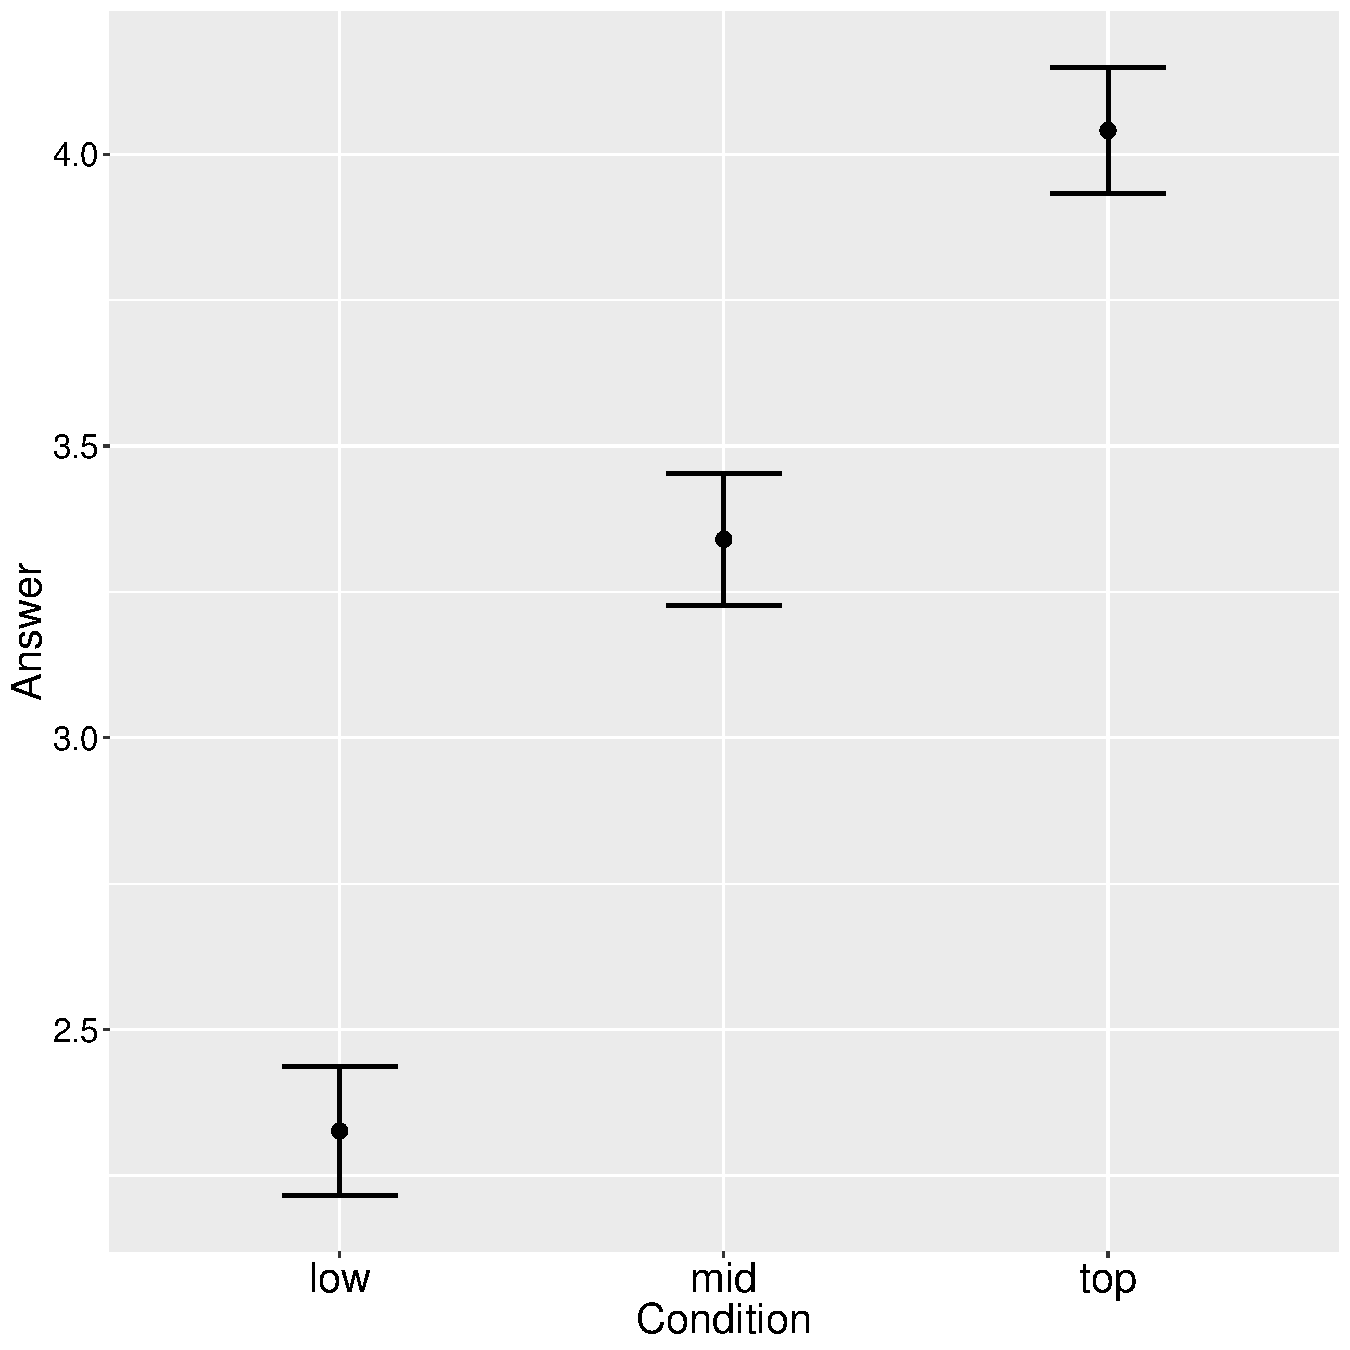
\includegraphics[scale=0.3]{exp1-part_1-errorbars.pdf}
\captionof{figure}{Error-bars, Experiment 1, part 1}
\end{center}

\end{frame}


\begin{frame}[fragile]

\tiny

\begin{Shaded}
\begin{Highlighting}[]
\NormalTok{Fixed effects}\OperatorTok{:}
\StringTok{             }\NormalTok{Estimate Std. Error       df t value }\KeywordTok{Pr}\NormalTok{(}\OperatorTok{>}\ErrorTok{|}\NormalTok{t}\OperatorTok{|}\NormalTok{)    }
\NormalTok{(Intercept)    }\FloatTok{3.3500}     \FloatTok{0.1915}  \FloatTok{14.2807}  \FloatTok{17.491} \FloatTok{4.80e-11} \OperatorTok{**}\ErrorTok{*}
\NormalTok{Conditionlow  }\OperatorTok{-}\FloatTok{1.0257}     \FloatTok{0.1415} \FloatTok{382.4998}  \OperatorTok{-}\FloatTok{7.246} \FloatTok{2.38e-12} \OperatorTok{**}\ErrorTok{*}
\NormalTok{Conditiontop   }\FloatTok{0.6831}     \FloatTok{0.1415} \FloatTok{382.4998}   \FloatTok{4.826} \FloatTok{2.02e-06} \OperatorTok{**}\ErrorTok{*}
\OperatorTok{---}
\NormalTok{Signif. codes}\OperatorTok{:}\StringTok{  }\DecValTok{0}\NormalTok{ ‘}\OperatorTok{**}\ErrorTok{*}\NormalTok{’ }\FloatTok{0.001}\NormalTok{ ‘}\OperatorTok{**}\NormalTok{’ }\FloatTok{0.01}\NormalTok{ ‘}\OperatorTok{*}\NormalTok{’ }\FloatTok{0.05}\NormalTok{ ‘.’ }\FloatTok{0.1}\NormalTok{ ‘ ’ }\DecValTok{1}

\NormalTok{Correlation of Fixed Effects}\OperatorTok{:}
\StringTok{            }\NormalTok{(Intr) Cndtnl}
\NormalTok{Conditionlw }\OperatorTok{-}\FloatTok{0.370}       
\NormalTok{Conditiontp }\OperatorTok{-}\FloatTok{0.370}  \FloatTok{0.500}
\OperatorTok{>}\StringTok{ }
\end{Highlighting}
\end{Shaded}

\normalsize

\begin{itemize}
\tightlist
\item
  reference level condition: \cond{mid} (releveled) -- all fixed effects
  significant
\item
  high preference for strong expressions associating with \emph{i}
\item
  middle: shrinking of the domain?
\end{itemize}

\end{frame}

\begin{frame}{Part 2}

\begin{center}
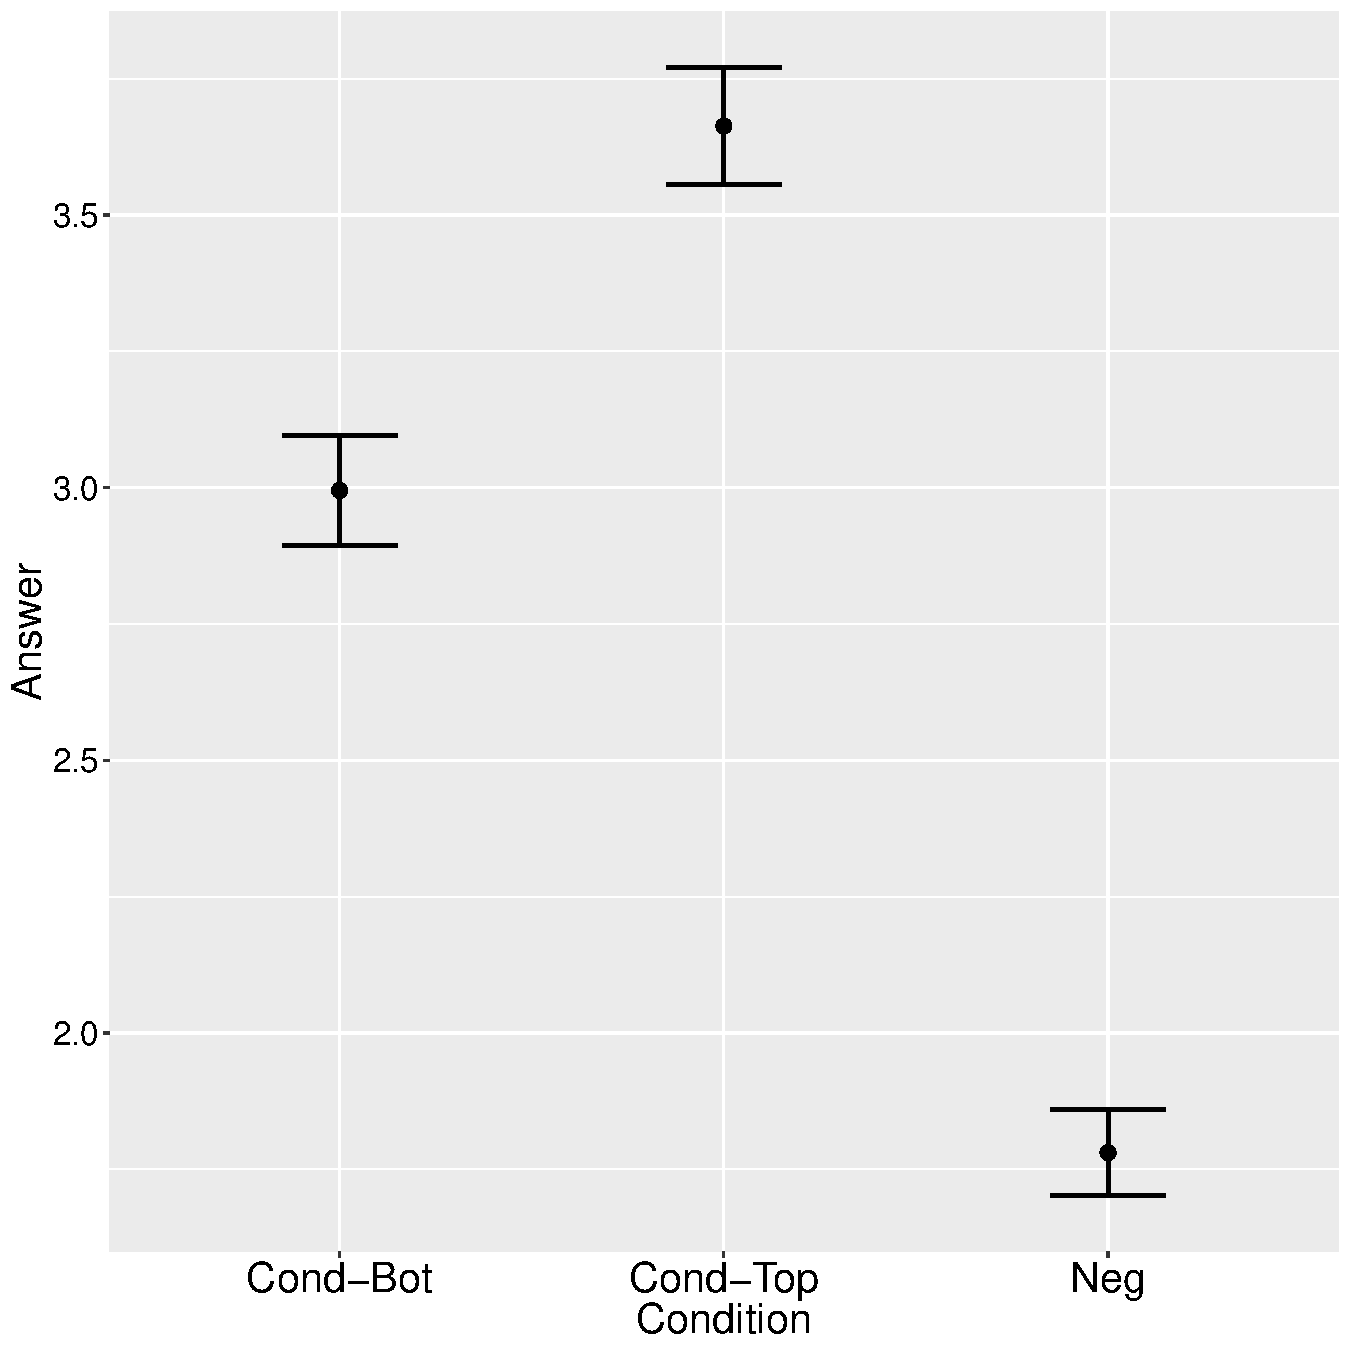
\includegraphics[scale=0.3]{exp1-part_2-errorbars.pdf}
\captionof{figure}{Error-bars, Experiment 1, part 2}
\end{center}

\end{frame}

\begin{frame}[fragile]

\tiny

\begin{Shaded}
\begin{Highlighting}[]
\NormalTok{Fixed effects}\OperatorTok{:}
\StringTok{                  }\NormalTok{Estimate Std. Error       df t value }\KeywordTok{Pr}\NormalTok{(}\OperatorTok{>}\ErrorTok{|}\NormalTok{t}\OperatorTok{|}\NormalTok{)    }
\NormalTok{(Intercept)         }\FloatTok{3.0210}     \FloatTok{0.1234} \FloatTok{112.5777}  \FloatTok{24.490}  \OperatorTok{<}\StringTok{ }\FloatTok{2e-16} \OperatorTok{**}\ErrorTok{*}
\NormalTok{ConditionCond}\OperatorTok{-}\NormalTok{Top   }\FloatTok{0.5883}     \FloatTok{0.1293} \FloatTok{515.7070}   \FloatTok{4.551} \FloatTok{6.66e-06} \OperatorTok{**}\ErrorTok{*}
\NormalTok{ConditionNeg       }\OperatorTok{-}\FloatTok{1.2590}     \FloatTok{0.1285} \FloatTok{531.0764}  \OperatorTok{-}\FloatTok{9.801}  \OperatorTok{<}\StringTok{ }\FloatTok{2e-16} \OperatorTok{**}\ErrorTok{*}
\OperatorTok{---}
\NormalTok{Signif. codes}\OperatorTok{:}\StringTok{  }\DecValTok{0}\NormalTok{ ‘}\OperatorTok{**}\ErrorTok{*}\NormalTok{’ }\FloatTok{0.001}\NormalTok{ ‘}\OperatorTok{**}\NormalTok{’ }\FloatTok{0.01}\NormalTok{ ‘}\OperatorTok{*}\NormalTok{’ }\FloatTok{0.05}\NormalTok{ ‘.’ }\FloatTok{0.1}\NormalTok{ ‘ ’ }\DecValTok{1}

\NormalTok{Correlation of Fixed Effects}\OperatorTok{:}
\StringTok{            }\NormalTok{(Intr) CndC}\OperatorTok{-}\NormalTok{T}
\NormalTok{CndtnCnd}\OperatorTok{-}\NormalTok{Tp }\OperatorTok{-}\FloatTok{0.521}       
\NormalTok{ConditionNg }\OperatorTok{-}\FloatTok{0.520}  \FloatTok{0.499}
\OperatorTok{>}\StringTok{ }
\end{Highlighting}
\end{Shaded}

\normalsize

\begin{itemize}
\tightlist
\item
  reference level: \cond{Cond-Bot}, the other two conditions are
  significantly different
\item
  again \emph{i} prefers to associate with strong elements but not so
  uncontroversially as in simple sentences
\end{itemize}

\end{frame}

\begin{frame}

\begin{itemize}
\tightlist
\item
  surprising: Strawson-Downward-Entailment (SDE) 
\end{itemize}

\ex. Even if John read ONE book, he will pass the exam. \a. even(C)(if
John read one book \ldots{}) is defined only if for all relevant
\emph{n} \textgreater{} 1: if John read one book \ldots{} \(<_c\) if
John read \emph{n} books \hfill (consistent)

\begin{itemize}
\tightlist
\item
  expected ungrammaticality (plus change of the predicate!) but reported
  as acceptable: Crnič (2012)
\end{itemize}

\ex. Even if John read ALL books, he will fail the exam. \a. even(C)(if
John read all books \ldots{}) is defined only if for all relevant
\emph{n} \textless{} \emph{all}: if John read all book \ldots{} \(<_c\)
if John read \emph{n} books \hfill (inconsistent)

\end{frame}



\begin{frame}{Summary}

\begin{itemize}
\tightlist
\item
  \emph{i} associates with strong elements even in the antecedent of
  conditional, ungrammatical in negated sentences (reference level conditions)
\end{itemize}

\ex. \a. \(\checkmark\) {[}\ldots{} \emph{i} + TOP \ldots{}{]}
\hfill Top \b. * \(\neg\){[}\ldots{} \emph{i} \ldots{}{]} \hfill Neg

\begin{itemize}
\tightlist
\item  \emph{i} can associate with weak elements in conditionals (decr. acc.)
\end{itemize}

\ex. \a. if {[}\ldots{} \emph{i} + TOP \ldots{}{]} \hfill Cond-Top \b.
{[}\ldots{} \emph{i} + MIDDLE \ldots{}{]} \hfill Mid \c. {[}\ldots{}
\emph{i} + BOTTOM \ldots{}{]} \hfill Cond-Bot \d. {[}\ldots{} \emph{i} +
LOW \ldots{}{]} \hfill Low

\end{frame}


\begin{frame}{Negative \emph{even} in Czech\\ Part 1}

\begin{itemize}
\tightlist
\item
  the same experiment 
\end{itemize}

\ex. Brown rice can preserve essential vitamins but \ldots{} it up to
three days after cooking.\label{ex-2} \a. Rýže v ledničce nevydrží
\textbf{ani} tři dny. \label{ex-1-a}\hfill (\cond{top})\newline
`The rice in the fridge doesn't last neg-even three days.' \b. Rýže v
ledničce nevydrží \textbf{ani} dva
dny.\label{ex-1-b}\hfill (\cond{mid})\newline
`The rice in the fridge doesn't last neg-even two days.' \c. Rýže v
ledničce nevydrží \textbf{ani} jeden
den.\hfill (\cond{low})\label{ex-1-c}\newline
`The rice in the fridge doesn't last neg-even one day.'

\end{frame}

\begin{frame}{Part 2}

\begin{itemize}
\tightlist
\item
  the same experiment 
\item
  selected conditions from the part 2:
\end{itemize}

\ex. Mother would be happy if her son would work for the police.
\ldots{} sergeant \ldots{} a colonel \ldots{} a general.\label{ex-3} \a.
Syn se nakonec nestal (\textbf{ani} rotným)/(\textbf{ani}
generálmajorem).\hfill (\cond{neg/neg-top}) \label{ex-3-a}\newline
`Son at the end didn't become neg-even (sergeant)/(general).' \b. Jestli
se syn stane \textbf{ani} rotným, bude matka
ráda.\hfill{(\cond{CondPos})}\label{ex-2-b}\newline
`If her son becomes neg-even sergeant, his mother would be happy.'

\end{frame}


\begin{frame}{Part 1}

\begin{center}
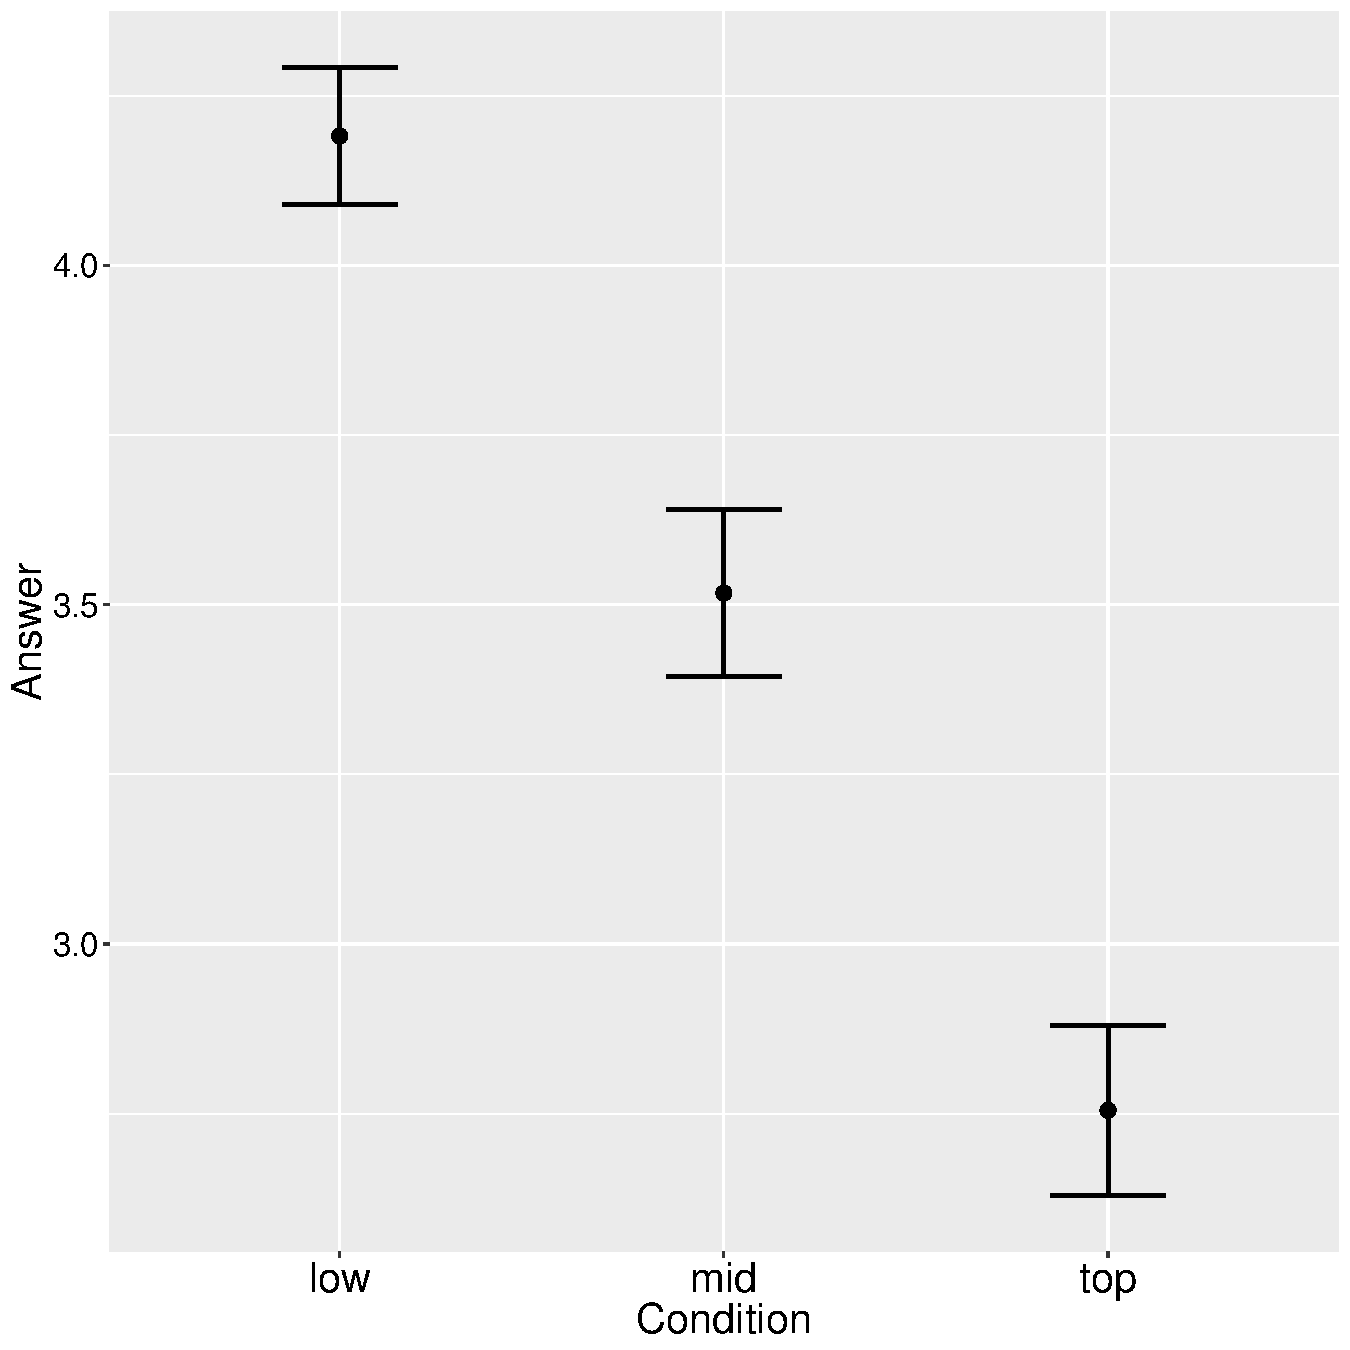
\includegraphics[scale=0.3]{exp1-ani-part_1-errorbars.pdf}
\captionof{figure}{Error-bars \textit{ani}, Experiment 1, part 1}
\end{center}

\end{frame}


\begin{frame}[fragile]

\tiny

\begin{Shaded}
\begin{Highlighting}[]
\NormalTok{Fixed effects}\OperatorTok{:}
\StringTok{             }\NormalTok{Estimate Std. Error       df t value }\KeywordTok{Pr}\NormalTok{(}\OperatorTok{>}\ErrorTok{|}\NormalTok{t}\OperatorTok{|}\NormalTok{)    }
\NormalTok{(Intercept)    }\FloatTok{3.4901}     \FloatTok{0.2020}  \FloatTok{16.7490}  \FloatTok{17.274} \FloatTok{4.17e-12} \OperatorTok{**}\ErrorTok{*}
\NormalTok{Conditionlow   }\FloatTok{0.7269}     \FloatTok{0.1445} \FloatTok{382.5049}   \FloatTok{5.031} \FloatTok{7.53e-07} \OperatorTok{**}\ErrorTok{*}
\NormalTok{Conditiontop  }\OperatorTok{-}\FloatTok{0.7346}     \FloatTok{0.1445} \FloatTok{382.5049}  \OperatorTok{-}\FloatTok{5.084} \FloatTok{5.79e-07} \OperatorTok{**}\ErrorTok{*}
\OperatorTok{---}
\NormalTok{Signif. codes}\OperatorTok{:}\StringTok{  }\DecValTok{0}\NormalTok{ ‘}\OperatorTok{**}\ErrorTok{*}\NormalTok{’ }\FloatTok{0.001}\NormalTok{ ‘}\OperatorTok{**}\NormalTok{’ }\FloatTok{0.01}\NormalTok{ ‘}\OperatorTok{*}\NormalTok{’ }\FloatTok{0.05}\NormalTok{ ‘.’ }\FloatTok{0.1}\NormalTok{ ‘ ’ }\DecValTok{1}

\NormalTok{Correlation of Fixed Effects}\OperatorTok{:}
\StringTok{            }\NormalTok{(Intr) Cndtnl}
\NormalTok{Conditionlw }\OperatorTok{-}\FloatTok{0.358}       
\NormalTok{Conditiontp }\OperatorTok{-}\FloatTok{0.358}  \FloatTok{0.500}
\OperatorTok{>}
\end{Highlighting}
\end{Shaded}

\normalsize

\begin{itemize}
\tightlist
\item
  reference level condition: \cond{mid} (releveled) -- all fixed again
  effects significant
\item
  high preference for weak expressions associating with \emph{ani}
\item
  middle: shrinking of the domain again?
\end{itemize}

\end{frame}

\begin{frame}{Part 2}

\begin{center}
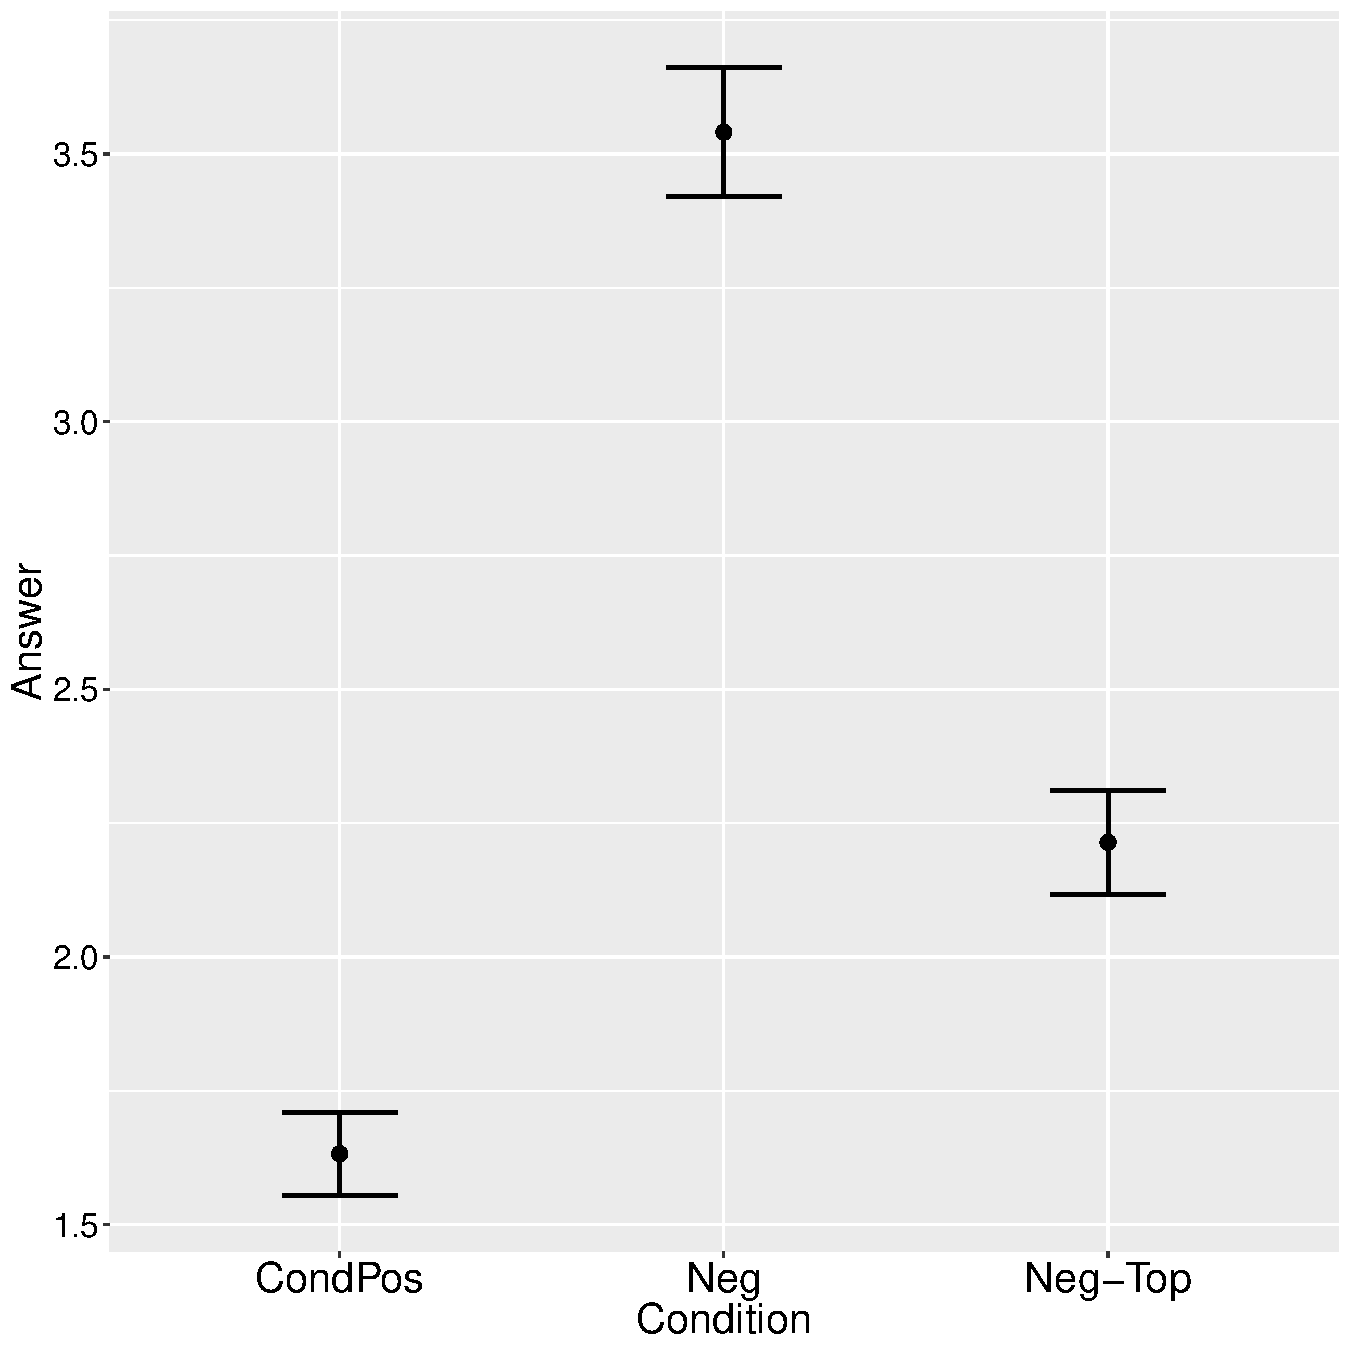
\includegraphics[scale=0.3]{exp1-ani-part_2-errorbars.pdf}
\captionof{figure}{Error-bars \textit{ani}, Experiment 1, part 2}
\end{center}

\end{frame}


\begin{frame}[fragile]

\tiny

\begin{Shaded}
\begin{Highlighting}[]
\NormalTok{Fixed effects}\OperatorTok{:}
\StringTok{                 }\NormalTok{Estimate Std. Error       df t value }\KeywordTok{Pr}\NormalTok{(}\OperatorTok{>}\ErrorTok{|}\NormalTok{t}\OperatorTok{|}\NormalTok{)    }
\NormalTok{(Intercept)        }\FloatTok{2.2084}     \FloatTok{0.1275}  \FloatTok{96.5876}  \FloatTok{17.326}  \OperatorTok{<}\StringTok{ }\FloatTok{2e-16} \OperatorTok{**}\ErrorTok{*}
\NormalTok{ConditionCondPos  }\OperatorTok{-}\FloatTok{0.5888}     \FloatTok{0.1377} \FloatTok{532.7231}  \OperatorTok{-}\FloatTok{4.275} \FloatTok{2.26e-05} \OperatorTok{**}\ErrorTok{*}
\NormalTok{ConditionNeg       }\FloatTok{1.2854}     \FloatTok{0.1367} \FloatTok{541.2981}   \FloatTok{9.404}  \OperatorTok{<}\StringTok{ }\FloatTok{2e-16} \OperatorTok{**}\ErrorTok{*}
\OperatorTok{---}
\NormalTok{Signif. codes}\OperatorTok{:}\StringTok{  }\DecValTok{0}\NormalTok{ ‘}\OperatorTok{**}\ErrorTok{*}\NormalTok{’ }\FloatTok{0.001}\NormalTok{ ‘}\OperatorTok{**}\NormalTok{’ }\FloatTok{0.01}\NormalTok{ ‘}\OperatorTok{*}\NormalTok{’ }\FloatTok{0.05}\NormalTok{ ‘.’ }\FloatTok{0.1}\NormalTok{ ‘ ’ }\DecValTok{1}

\NormalTok{Correlation of Fixed Effects}\OperatorTok{:}
\StringTok{            }\NormalTok{(Intr) CndtCP}
\NormalTok{CondtnCndPs }\OperatorTok{-}\FloatTok{0.536}       
\NormalTok{ConditionNg }\OperatorTok{-}\FloatTok{0.536}  \FloatTok{0.499}
\OperatorTok{>}\StringTok{ }
\end{Highlighting}
\end{Shaded}

\normalsize

\begin{itemize}
\tightlist
\item
  reference level: \cond{Neg-Top}, the other two conditions are
  significantly different
\item
  again \emph{ani} prefers to associate with weak elements (Neg
  \textgreater{} Neg-Top)
\item
  Strawson-DE is not enough to license it (CondPos)
\end{itemize}

\end{frame}


\begin{frame}{Summary \emph{ani}}

\begin{itemize}
\tightlist
\item
  \emph{ani} behaves more according to Krifka's theory
\item
  association nearly only with weak elements (scope over negation)
\item
  association with strong elements only marginal (\cond{Top}) or
  un-acceptable (\cond{Neg-Top})
\item
  direct comparison with \emph{i} hard: \emph{i} in negated sentences is
  blocked by \emph{ani}
\item
  theoretical explanation: \emph{ani} cannot scope over exh (?)
\end{itemize}

\end{frame}

\begin{frame}{Summary \emph{i} + \emph{ani}}

\begin{enumerate}
\def\labelenumi{\arabic{enumi})}
\tightlist
\item
  \emph{i}: positive \emph{even}, associates with strong elements

  \begin{itemize}
  \tightlist
  \item
    evidence for scope \emph{even} theories: acceptability of both
    scalar end association (conditional)
  \item
    hard to explain in ambiguity approaches: \emph{i} is only the
    positive \emph{even}
  \item
    evidence for embedded exhaustification: strong association preferred
    even in conditionals
  \item
    evidence for PPI behaviour (limited: weak assoc. in conditionals)
  \end{itemize}
\end{enumerate}

\end{frame}

\begin{frame}

\begin{enumerate}
\def\labelenumi{\arabic{enumi})}
\setcounter{enumi}{1}
\tightlist
\item
  \emph{ani}: negative \emph{even}, associates with weak elements

  \begin{itemize}
  \tightlist
  \item
    evidence for scope theories (limited: marginal ambiguity in negated
    sentences)
  \item
    no evidence for embedded exhaustification
  \item
    evidence for PPI behaviour of covert \emph{even}: strong preference
    of weak elements
  \end{itemize}
\end{enumerate}

\end{frame}

\begin{frame}{Interpretation}

\begin{itemize}
\tightlist
\item
  \emph{i}: Czech positive \emph{even} with the un-likelihood
  presupposition
\item
  explains: high acceptability of Top, low acceptability of Low
\item
  ungrammaticality with Neg (different source: concurrence)
\item
  PPI hypothesis predicts unobserved preference of the Cond-Bot over
  Cond-Top
\end{itemize}

\end{frame}

\begin{frame}

\begin{itemize}
\tightlist
\item
  explanation (after Crnič (2012)): expected \emph{even}-association
  with weak elements \Next (in DE contexts 1 \(\rightarrow\) 2,
  \ldots{})
\item
  but unexpected \emph{even}-association with strong elements \NNext:
\item
  problem: truth of \emph{if John \(\exists\) he \ldots{}}
  \(\rightarrow\) \emph{If John \(\forall\) he \ldots{}}
\item
  \(\forall\) cannot be less likely than \(\exists\)
\end{itemize}

\ex. Even if John read ONE book, he will pass the exam. \a. even(C)(if
John read one book \ldots{}) is defined only if for all relevant
\emph{n} \textgreater{} 1: if John read one book \ldots{} \(<_c\) if
John read \emph{n}-books \hfill (trivial)

\ex. Even if John read ALL of the books, he will fail the exam.
\a.even(C)(if John read all books \ldots{}) is defined only if John read
all books \ldots{} \(<_c\) if John read some books \ldots{}
\hfill (inconsistent)

\end{frame}

\begin{frame}

Crnič's solution:

\begin{itemize}
\tightlist
\item
  exhaustification
\item
  the alternatives are then \Next[a], not \Next[b]
\end{itemize}

\ex. {[}even C\(_2\){]} {[}if {[}exh C\(_0\){]} {[}John read all\(_F\)
of the books{]} he will fail the exam{]} \a. \{that if John read all of
the books he will FTE, that if John read some but not all of the books
he will FTE\} \b. \{that if John read all of the books he will FTE, that
if John read some of the books he will FTE\}

\ex. exh(C)(p,w) = 1 iff p(w)=1 and
\(\forall q\in C[p \not\subseteq q \rightarrow q(w) = 0]\)\newline
all the alternatives not entailed by the prejacent are false

\end{frame}

\begin{frame}

\begin{itemize}
\tightlist
\item
  applied to the experiment
\item
  logically (and not even contextually) un-ordered/independent
\item
  likelihood of logically independent alternatives un-constrained
\item
  plausible context: correlation of son's achieved rank with his mother
  happiness
\end{itemize}

\ex. {[}even C\(_2\){]} {[}if {[}exh C\(_0\){]} {[}son becomes
general\(_F\){]} mother will be happy{]} \a. \{that if son becomes
general mother will be happy, that if son becomes mayor and not general
mother will be happy, that if son becomes sergeant and not general
mother will be happy\}

\end{frame}

\begin{frame}

Conclusion

\begin{itemize}
\tightlist
\item
  \emph{i} can have wide scope (PPI) and associate with strong elements
\item
  PPI properties masked by the exhaustification
\end{itemize}

\ex. Prediction: the environments where the exhaustification is blocked
or weakened shouldn't allow association of \emph{even} with strong
elements.


\end{frame}

\begin{frame}{Summary and questions}

\begin{enumerate}
\def\labelenumi{\arabic{enumi})}
\item
	scalar properties of \textit{i}/\textit{ani} described in Crnič's framework $\checkmark$
\item
	\textit{i} scopal (both ends of scales accept.), \textit{ani} associates only with weak elements (marginal acceptability of \textbf{Top})
\item Future work: additivity + scope theories: 
\end{enumerate}

\ex. Parents neg-allowed Petr go \textbf{ani} to boy-scout.
\a. local presupposition: Petr didn't go to ALT(boy-scout) ... movies, ... \hfill NPI presupp.
\b. global: Parents neg-allowed Petr to ALT(boy-scout) ... movies, ... \hfill scope presupp.

\end{frame}

\begin{frame}

\begin{center}
\Huge Thanks!
\end{center}

\end{frame}

\begin{frame}{Appendix}

\begin{itemize}
\tightlist
\item
  note: the environments (conditionals, restriction of plural definites
  and universal quantifiers) are Strawson-downward entailing:
\end{itemize}

\ex. \a. If son will become sergeant his mom will be happy.\newline
\(\approx \forall w \in Acc\){[}son becomes seregant in \emph{w}
\(\rightarrow\) mom happy in \emph{w}{]} \b. It is possible that son
will become mayor or more. \c. \{w: son become mayor or more in
\emph{w}\} \(\subseteq\) \{w: son will become sergeant in \emph{w}\} \d.
\(\models\) If son will become general his mom will be happy.\newline
\(\approx \forall w \in Acc\){[}son becomes general in \emph{w}
\(\rightarrow\) mom happy in \emph{w}{]}

\end{frame}

\begin{frame}{All conditions together}

\begin{center}
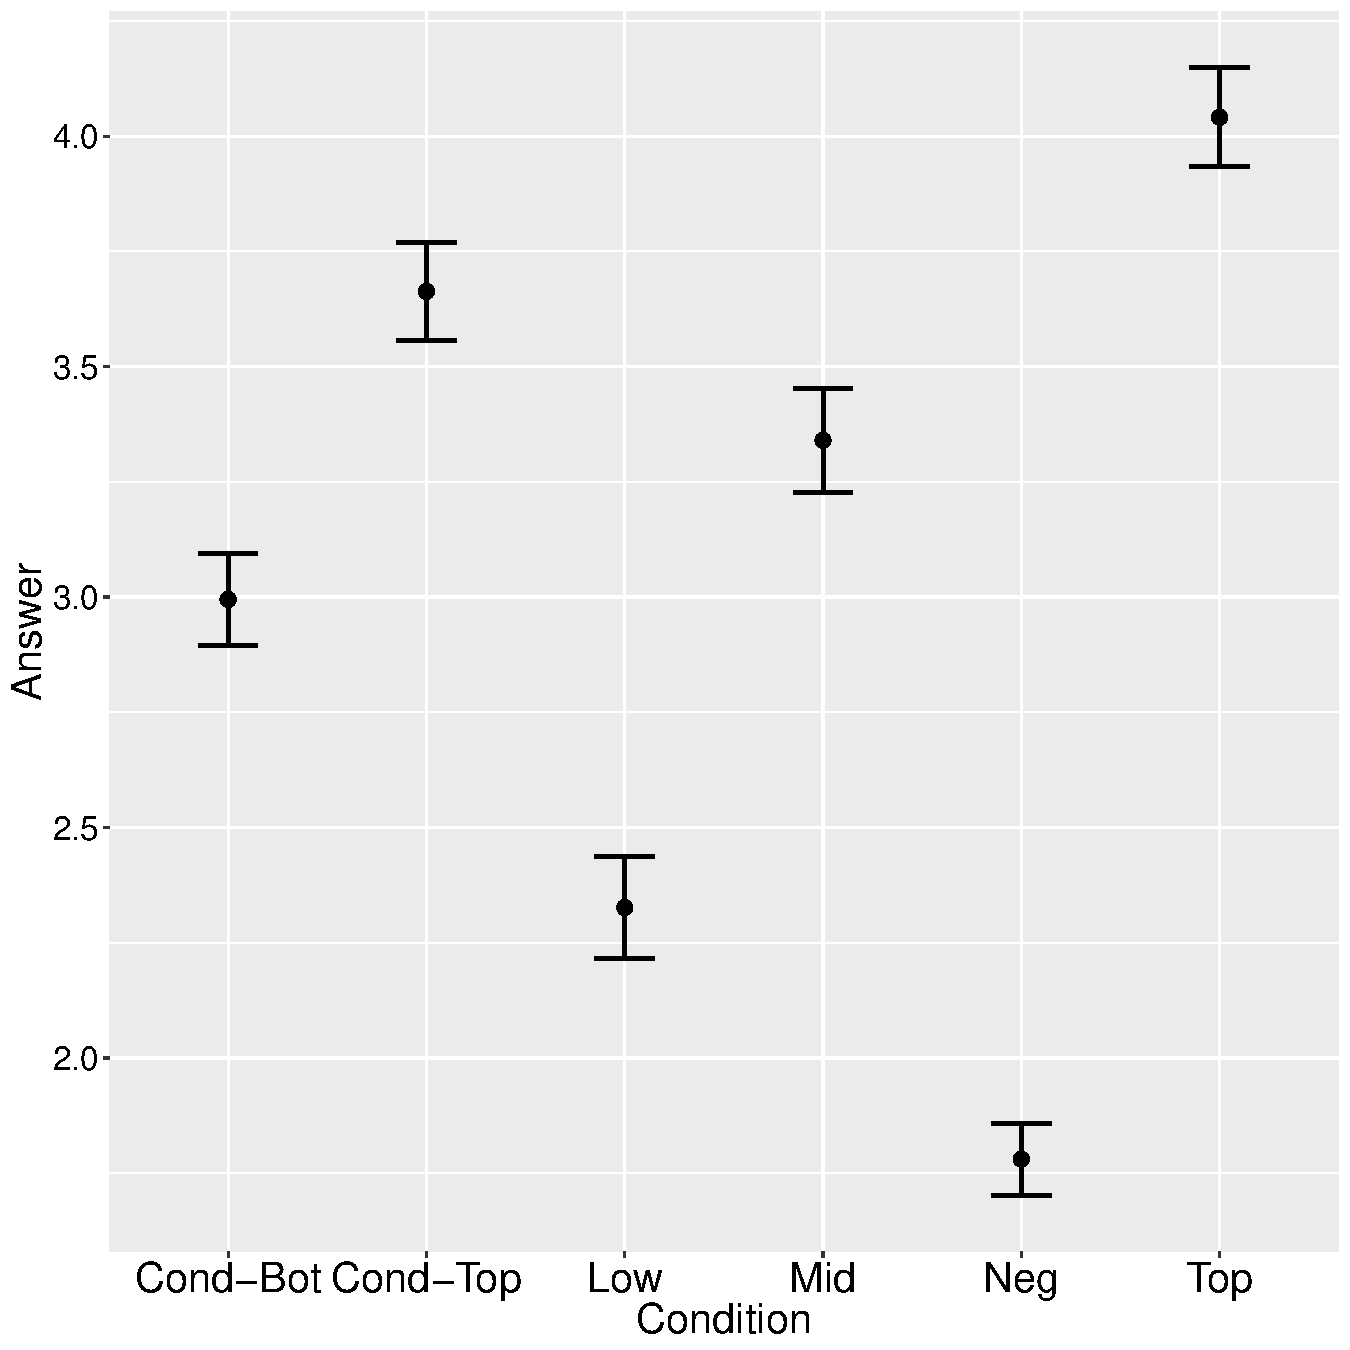
\includegraphics[scale=0.3]{exp1-part_1-2-errorbars.pdf}
\captionof{figure}{Error-bars, Experiment 1, all conditions}
\end{center}

\end{frame}

\begin{frame}{All conditions together}

\begin{center}
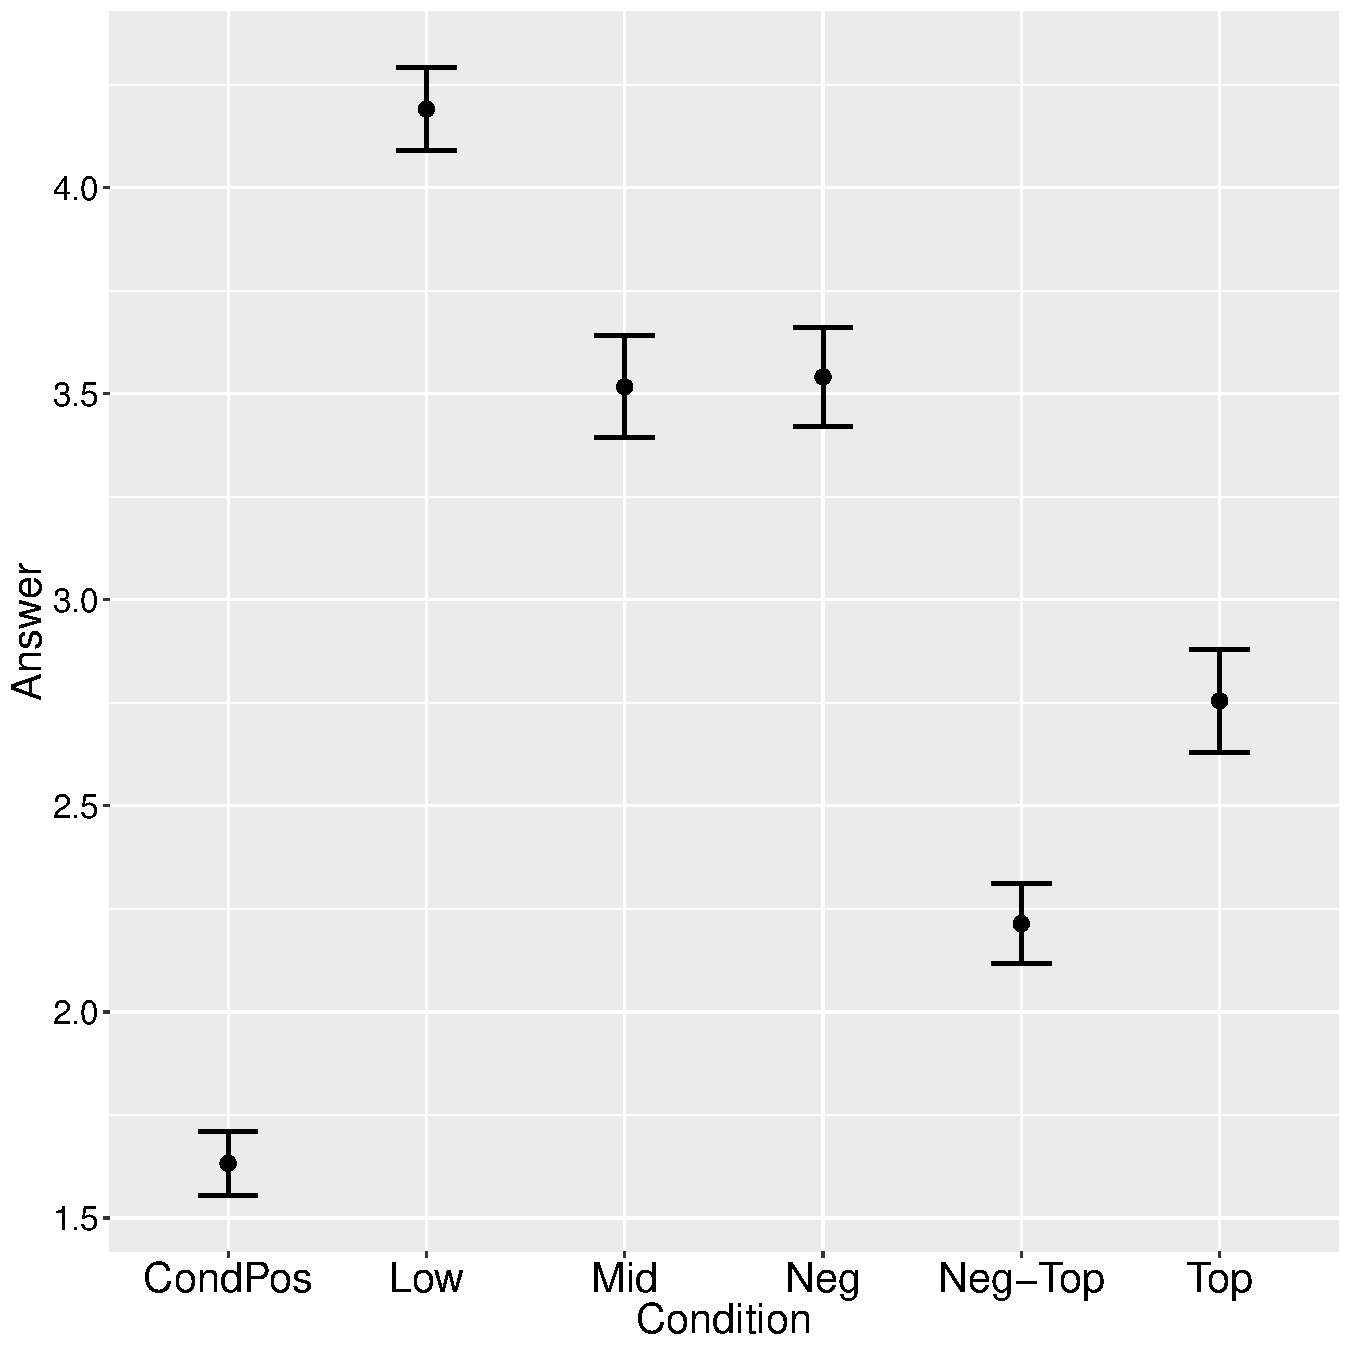
\includegraphics[scale=0.3]{exp1-ani-part_1-2-errorbars.pdf}
\captionof{figure}{Error-bars, Experiment 1 \textit{ani}, all conditions}
\end{center}

\end{frame}


\begin{frame}

Crnič (2012) (exhaustified \Next[a] \emph{read some but not all} would
be non-contradictory):

\ex. \a. ?I doubt that John read some of the books but I also doubt that
he read all of the books. \b. ?I even doubt that John read ALL of the
books.


\begin{itemize}
\tightlist
\item
  contrast this with obligatory exhaustification (\emph{read some but
  not all}):
\end{itemize}

\ex. The students who read some of the books failed the exam but also
the students who read all of the books did.

\begin{itemize}
\tightlist
\item
  to be tested
\item
  plus: only in exhaustified cases a change of predicate should have an
  effect (\emph{even ONE} vs. \emph{ANY})
\end{itemize}
\end{frame}

\begin{frame}{\emph{ani} vs.~n-words}

Previous experiments (with Jakub Dotlačil):

\begin{itemize}
\tightlist
\item
  \emph{ani} is licensed in semantics, not in syntax
\item
  does not behave like n-word
\item
  in previous experiments: positive interaction of \emph{ani} and NR
\item
  typical items (acceptability judgments: contrast between n-words --
  \emph{žádný}, \ldots{} and \emph{ani})
\end{itemize}

\ex. \a. ?Nechci, aby ani jeden student vyletěl.\newline
 neg-want.1SG COMP neg-even one student failed \b. ??Nechci, aby žádný
student vyletěl.\newline
 neg-want.1SG COMP n-word student failed

\end{frame}

\begin{frame}

\begin{longtable}[]{@{}lll@{}}
\toprule
environment/status & NPIs & n-words\tabularnewline
\midrule
\endhead
NR embedded & \(\checkmark\) & X\tabularnewline
non NR embedded & X & X\tabularnewline
\bottomrule
\end{longtable}

\end{frame}

\begin{frame}

\begin{center}
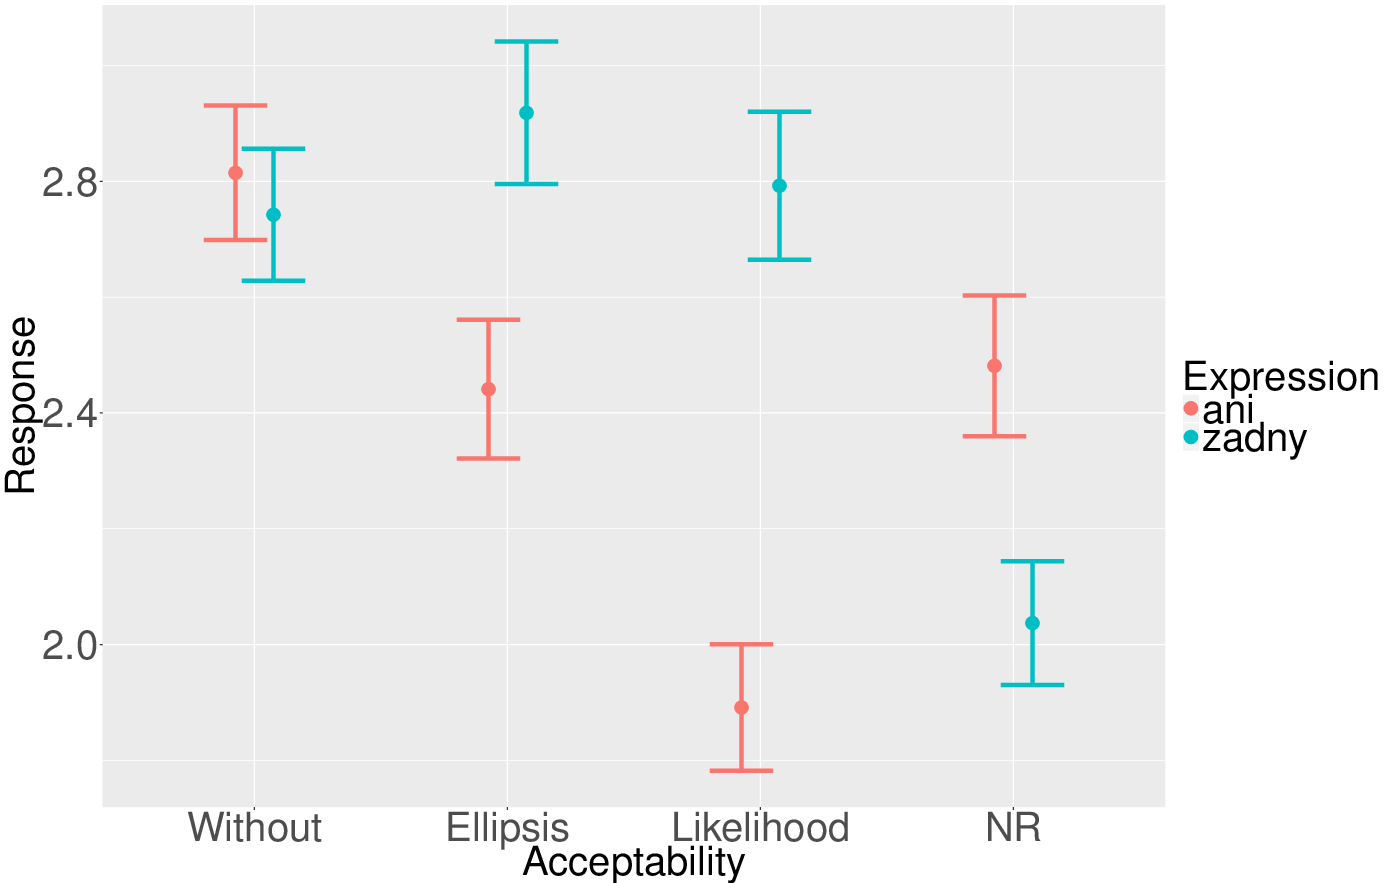
\includegraphics[scale=0.23]{mean-sum.png}
\captionof{figure}{\textit{ani} vs. n-words}
\end{center}

\end{frame}

\begin{frame}[fragile]{PPI-exp: Descriptive statistics for part 1}

\tiny 

\begin{Shaded}
\begin{Highlighting}[]
\OperatorTok{>}\StringTok{ }\KeywordTok{ddply}\NormalTok{(data_ppi, .(Condition), summarise, }\DataTypeTok{Means =} \KeywordTok{mean}\NormalTok{(Answer, }\DataTypeTok{na.rm=}\OtherTok{TRUE}\NormalTok{))}
\NormalTok{  Condition    Means}
\DecValTok{1}\NormalTok{  Cond}\OperatorTok{-}\NormalTok{Bot }\FloatTok{2.994898}
\DecValTok{2}\NormalTok{  Cond}\OperatorTok{-}\NormalTok{Top }\FloatTok{3.663265}
\DecValTok{3}\NormalTok{       Low }\FloatTok{2.326531}
\DecValTok{4}\NormalTok{       Mid }\FloatTok{3.340136}
\DecValTok{5}\NormalTok{       Neg }\FloatTok{1.780612}
\DecValTok{6}\NormalTok{       Top }\FloatTok{4.040816}
\OperatorTok{>}\StringTok{ }\KeywordTok{ddply}\NormalTok{(data_ppi, .(Condition), summarise, }\DataTypeTok{Medians =} \KeywordTok{median}\NormalTok{(Answer,}\DataTypeTok{na.rm=}\OtherTok{TRUE}\NormalTok{))}
\NormalTok{  Condition Medians}
\DecValTok{1}\NormalTok{  Cond}\OperatorTok{-}\NormalTok{Bot       }\DecValTok{3}
\DecValTok{2}\NormalTok{  Cond}\OperatorTok{-}\NormalTok{Top       }\DecValTok{4}
\DecValTok{3}\NormalTok{       Low       }\DecValTok{2}
\DecValTok{4}\NormalTok{       Mid       }\DecValTok{4}
\DecValTok{5}\NormalTok{       Neg       }\DecValTok{1}
\DecValTok{6}\NormalTok{       Top       }\DecValTok{5}
\OperatorTok{>}\StringTok{ }
\end{Highlighting}
\end{Shaded}

\end{frame}

\begin{frame}[fragile]{PPI-exp: Linear mixed model for part 1}

\begin{itemize}
\tightlist
\item
  package \emph{lmerTest} (\emph{p} value info)
\end{itemize}

\tiny

\begin{Shaded}
\begin{Highlighting}[]
\OperatorTok{>}\StringTok{ }\NormalTok{m1 <-}\StringTok{ }\KeywordTok{lmer}\NormalTok{(}\KeywordTok{as.numeric}\NormalTok{(Answer) }\OperatorTok{~}\StringTok{ }\NormalTok{Condition }\OperatorTok{+}\StringTok{ }\NormalTok{(}\DecValTok{1}\OperatorTok{|}\NormalTok{Subj) }\OperatorTok{+}\StringTok{ }\NormalTok{(}\DecValTok{1}\OperatorTok{|}\NormalTok{Item), }\DataTypeTok{data=}\NormalTok{data_ppi_}\DecValTok{1}\NormalTok{)}
\OperatorTok{>}\StringTok{ }\KeywordTok{summary}\NormalTok{(m1)}
\NormalTok{Linear mixed model fit by REML. t}\OperatorTok{-}\NormalTok{tests use Satterthwaite}\StringTok{'s method ['}\NormalTok{lmerModLmerTest}\StringTok{']}
\StringTok{Formula: as.numeric(Answer) ~ Condition + (1 | Subj) + (1 | Item)}
\StringTok{   Data: data_ppi_1}

\StringTok{REML criterion at convergence: 1470.5}

\StringTok{Scaled residuals: }
\StringTok{    Min      1Q  Median      3Q     Max }
\StringTok{-3.1454 -0.7445  0.1116  0.7417  2.2667 }

\StringTok{Random effects:}
\StringTok{ Groups   Name        Variance Std.Dev.}
\StringTok{ Subj     (Intercept) 0.1307   0.3615  }
\StringTok{ Item     (Intercept) 0.2161   0.4649  }
\StringTok{ Residual             1.4656   1.2106  }
\StringTok{Number of obs: 441, groups:  Subj, 49; Item, 9}
\end{Highlighting}
\end{Shaded}

\end{frame}

\begin{frame}[fragile]{PPI-exp: Linear model for part 2}

\tiny

\begin{Shaded}
\begin{Highlighting}[]
\OperatorTok{>}\StringTok{ }\NormalTok{m1 <-}\StringTok{ }\KeywordTok{lmer}\NormalTok{(}\KeywordTok{as.numeric}\NormalTok{(Answer) }\OperatorTok{~}\StringTok{ }\NormalTok{Condition }\OperatorTok{+}\StringTok{ }\NormalTok{(}\DecValTok{1}\OperatorTok{|}\NormalTok{Subj) }\OperatorTok{+}\StringTok{ }\NormalTok{(}\DecValTok{1}\OperatorTok{|}\NormalTok{Item), }\DataTypeTok{data=}\NormalTok{data_ppi_}\DecValTok{2}\NormalTok{)}
\OperatorTok{>}\StringTok{ }\KeywordTok{summary}\NormalTok{(m1)}
\NormalTok{Linear mixed model fit by REML. t}\OperatorTok{-}\NormalTok{tests use Satterthwaite}\StringTok{'s method ['}\NormalTok{lmerModLmerTest}\StringTok{']}
\StringTok{Formula: as.numeric(Answer) ~ Condition + (1 | Subj) + (1 | Item)}
\StringTok{   Data: data_ppi_2}

\StringTok{REML criterion at convergence: 1982.9}

\StringTok{Scaled residuals: }
\StringTok{    Min      1Q  Median      3Q     Max }
\StringTok{-2.2804 -0.6559 -0.0431  0.7140  3.4371 }

\StringTok{Random effects:}
\StringTok{ Groups   Name        Variance Std.Dev.}
\StringTok{ Subj     (Intercept) 0.22450  0.4738  }
\StringTok{ Item     (Intercept) 0.07654  0.2767  }
\StringTok{ Residual             1.50289  1.2259  }
\StringTok{Number of obs: 588, groups:  Subj, 49; Item, 32}
\end{Highlighting}
\end{Shaded}

\end{frame}

\begin{frame}[fragile]{NPI-exp: Descriptive statistics}

\tiny 

\begin{Shaded}
\begin{Highlighting}[]
\OperatorTok{>}\StringTok{ }\KeywordTok{ddply}\NormalTok{(data_ani, .(Condition), summarise, }\DataTypeTok{Means =} \KeywordTok{mean}\NormalTok{(Answer, }\DataTypeTok{na.rm=}\OtherTok{TRUE}\NormalTok{))}
\NormalTok{  Condition    Means}
\DecValTok{1}\NormalTok{   CondPos }\FloatTok{1.632653}
\DecValTok{2}\NormalTok{       Low }\FloatTok{4.190476}
\DecValTok{3}\NormalTok{       Mid }\FloatTok{3.517007}
\DecValTok{4}\NormalTok{       Neg }\FloatTok{3.540816}
\DecValTok{5}\NormalTok{   Neg}\OperatorTok{-}\NormalTok{Top }\FloatTok{2.214286}
\DecValTok{6}\NormalTok{       Top }\FloatTok{2.755102}
\OperatorTok{>}\StringTok{ }\KeywordTok{ddply}\NormalTok{(data_ani, .(Condition), summarise, }\DataTypeTok{Medians =} \KeywordTok{median}\NormalTok{(Answer,}\DataTypeTok{na.rm=}\OtherTok{TRUE}\NormalTok{))}
\NormalTok{  Condition Medians}
\DecValTok{1}\NormalTok{   CondPos       }\DecValTok{1}
\DecValTok{2}\NormalTok{       Low       }\DecValTok{5}
\DecValTok{3}\NormalTok{       Mid       }\DecValTok{4}
\DecValTok{4}\NormalTok{       Neg       }\DecValTok{5}
\DecValTok{5}\NormalTok{   Neg}\OperatorTok{-}\NormalTok{Top       }\DecValTok{2}
\DecValTok{6}\NormalTok{       Top       }\DecValTok{3}
\OperatorTok{>}\StringTok{ }
\end{Highlighting}
\end{Shaded}

\end{frame}

\begin{frame}[fragile]{NPI-exp: Linear mixed model for part 1}

\tiny

\begin{Shaded}
\begin{Highlighting}[]
\OperatorTok{>}\StringTok{ }\NormalTok{m1 <-}\StringTok{ }\KeywordTok{lmer}\NormalTok{(}\KeywordTok{as.numeric}\NormalTok{(Answer) }\OperatorTok{~}\StringTok{ }\NormalTok{Condition }\OperatorTok{+}\StringTok{ }\NormalTok{(}\DecValTok{1}\OperatorTok{|}\NormalTok{Subj) }\OperatorTok{+}\StringTok{ }\NormalTok{(}\DecValTok{1}\OperatorTok{|}\NormalTok{Item), }\DataTypeTok{data=}\NormalTok{data_ani_}\DecValTok{1}\NormalTok{)}
\OperatorTok{>}\StringTok{ }\KeywordTok{summary}\NormalTok{(m1)}
\NormalTok{Linear mixed model fit by REML. t}\OperatorTok{-}\NormalTok{tests use Satterthwaite}\StringTok{'s method ['}\NormalTok{lmerModLmerTest}\StringTok{']}
\StringTok{Formula: as.numeric(Answer) ~ Condition + (1 | Subj) + (1 | Item)}
\StringTok{   Data: data_ani_1}

\StringTok{REML criterion at convergence: 1508}

\StringTok{Scaled residuals: }
\StringTok{    Min      1Q  Median      3Q     Max }
\StringTok{-2.9104 -0.7829  0.1487  0.7275  2.3556 }

\StringTok{Random effects:}
\StringTok{ Groups   Name        Variance Std.Dev.}
\StringTok{ Subj     (Intercept) 0.2906   0.5391  }
\StringTok{ Item     (Intercept) 0.2202   0.4693  }
\StringTok{ Residual             1.5272   1.2358  }
\StringTok{Number of obs: 441, groups:  Subj, 49; Item, 9}
\end{Highlighting}
\end{Shaded}

\end{frame}

\begin{frame}[fragile]{NPI-exp: Linear model for part 2}

\tiny

\begin{Shaded}
\begin{Highlighting}[]
\OperatorTok{>}\StringTok{ }\NormalTok{m1 <-}\StringTok{ }\KeywordTok{lmer}\NormalTok{(}\KeywordTok{as.numeric}\NormalTok{(Answer) }\OperatorTok{~}\StringTok{ }\NormalTok{Condition }\OperatorTok{+}\StringTok{ }\NormalTok{(}\DecValTok{1}\OperatorTok{|}\NormalTok{Subj) }\OperatorTok{+}\StringTok{ }\NormalTok{(}\DecValTok{1}\OperatorTok{|}\NormalTok{Item), }\DataTypeTok{data=}\NormalTok{data_ani_}\DecValTok{2}\NormalTok{)}
\OperatorTok{>}\StringTok{ }\KeywordTok{summary}\NormalTok{(m1)}
\NormalTok{Linear mixed model fit by REML. t}\OperatorTok{-}\NormalTok{tests use Satterthwaite}\StringTok{'s method ['}\NormalTok{lmerModLmerTest}\StringTok{']}
\StringTok{Formula: as.numeric(Answer) ~ Condition + (1 | Subj) + (1 | Item)}
\StringTok{   Data: data_ani_2}

\StringTok{REML criterion at convergence: 2042.3}

\StringTok{Scaled residuals: }
\StringTok{    Min      1Q  Median      3Q     Max }
\StringTok{-2.0527 -0.6597 -0.1860  0.7913  2.6439 }

\StringTok{Random effects:}
\StringTok{ Groups   Name        Variance Std.Dev.}
\StringTok{ Subj     (Intercept) 0.1643   0.4054  }
\StringTok{ Item     (Intercept) 0.1138   0.3373  }
\StringTok{ Residual             1.6856   1.2983  }
\StringTok{Number of obs: 588, groups:  Subj, 49; Item, 32}
\end{Highlighting}
\end{Shaded}

\end{frame}

\begin{frame}{Where to go}

\begin{enumerate}
\def\labelenumi{\arabic{enumi})}
\tightlist
\item
  check Crnič's predictions
\end{enumerate}

\begin{itemize}
\tightlist
\item
  correlation between the strength of the exhaustification \&
  possibility of strong \emph{even}
\item
  change of linearization!
\end{itemize}

\ex. time/irrealis(?) Czech if \a. Když splníš některé úkoly
(=\(\exists \vee \forall\)), tak projdeš.\\
when fulfill.2SG.FUT some tasks then succeed.2SG.FUT (no exh.) \b. I
když uděláš ?všechny úkoly, tak propadneš.\\
i when fulfill.2SG.FUT all tasks then fail.2SG.FUT

\end{frame}

\begin{frame}

\begin{itemize}
\tightlist
\item
  interesting observation: \emph{i} (unlike \emph{ani}) cannot directly
  modify universal quantifier (only in the \emph{even if} construction):
\end{itemize}

\ex. \a. Petr přečetl i třetí/??všechny díly PP.\\
Petr read i third/all volumes LOTR. \b. I když přečteš všechny díly PP,
nebudeš tolkienovský odborník.\\
Even when you-read all volumes LOTR, neg-will-become Tolkien expert.

\begin{itemize}
\tightlist
\item
  is it really association with \emph{all}?
\item
  if not how about original Crnič's examples?
\end{itemize}

\end{frame}

\begin{frame}

\begin{enumerate}
\def\labelenumi{\arabic{enumi})}
\setcounter{enumi}{1}
\tightlist
\item
  additivity presupposition
\end{enumerate}

\begin{itemize}
\tightlist
\item
  \emph{i}'s additivity presupp. is much stronger than English (Rullmann
  1997, ex.(18)):
\item
  cannot be NPI-\emph{even} (neither in English)
\end{itemize}

\ex. \a. A: Is Claire an ASSISTANT professor? \b. B: No, she's even an
ASSOCIATE professor.

\ex. \a. Klára je doktor? \b. ??Ne, one je i docent.\\
\ldots{} plausible only: another academic degree

\end{frame}

\begin{frame}

Crnič's observation: English addititivity presupp. depends on the
surface scope

\ex. \a. John is sorry that he even OPENED the book. \a. no additive
presupp. (read, \ldots{}) \z. \b. John is even sorry that he OPENED the
book. \a. additive presupp. (John read, \ldots{}) \z.

\end{frame}

\begin{frame}

Czech data: reversed (but the only grammatical case with \emph{když}
`when')

\begin{itemize}
\tightlist
\item
  Czech (similarly to German) usually requires adjacency of focus
  sensitive particles to FOC
\end{itemize}

\ex. \a. Petr si přečetl i třetí díl PP. \hfill +additive\\
Petr read i third volume LOTR. \b. I když si přečteš třetí díl PP, tak
první dva nečti. \hfill -additive\\
Even when you read third volume LOTR, then don't read the first two.

\ex. \a. Petr lituje, že přečetl i třetí díl PP.\\
Petr regrets that read.3SG i third volume LOTR. \b. Petr ??i lituje, že
přečetl třetí díl PP.

\end{frame}

\begin{frame}

\begin{enumerate}
\def\labelenumi{\arabic{enumi})}
\setcounter{enumi}{2}
\tightlist
\item
  project with Viola in Vienna
\end{enumerate}

\begin{itemize}
\tightlist
\item
  \emph{i} as obligatory? distributive conjunction
\end{itemize}

\ex. subject vs.~object \a. Klára i Bára namalovali 3 portéty.
\hfill +distr\\
Klára i Bára painted 3 portraits. \b. Petr, Karel a Martin pozvali Kláru
i Báru na své narozeniny. \hfill ?distr\\
Petr, Karel and Martin invited Klara i Bara \ldots{} \a. Petr
-\textgreater{} Klára \b. Karel -\textgreater{} Bára \c. Martin
-\textgreater{} Bára \z.

\end{frame}

\begin{frame}

\begin{itemize}
\tightlist
\item
  PPI behaviour in all syntactic configurations?
\end{itemize}

\ex. \a. Petr i Karel nepřišli.\\
Petr i Karel neg-arrived.\\
\(\neg p \wedge \neg k\) \b. Na své narozeniny jsem nepozval Petra i
Karla.\\
I didn't invite (for my birthday) Petr i Karel.\\
?\(\neg(p \wedge k)\)

\end{frame}

\begin{frame}{References I}

\scriptsize

\hypertarget{refs}{}
\hypertarget{ref-cohen2014superlative}{}
Cohen, Ariel, and Manfred Krifka. 2014. Superlative quantifiers and
meta-speech acts. \emph{Linguistics and Philosophy} 37. Springer:
41--90.

\hypertarget{ref-crnic2011getting}{}
Crnič, Luka. 2011. Getting even. PhD thesis, MIT.

\hypertarget{ref-crnivc2012focus}{}
Crnič, Luka. 2012. Focus particles and embedded exhaustification.
\emph{Journal of semantics} 30. Oxford University Press: 533--558.

\hypertarget{ref-crnivc2014against}{}
Crnič, Luka. 2014. Against a dogma on npi licensing. \emph{The art and
craft of semantics: A festschrift for Irene Heim} 1: 117--145.

\hypertarget{ref-giannakidou2007landscape}{}
Giannakidou, Anastasia. 2007. The landscape of even. \emph{Natural
Language \& Linguistic Theory} 25. Springer: 39--81.

\hypertarget{ref-heim1984note}{}
Heim, Irene. 1984. A note on negative polarity and downward
entailingness. In \emph{Proceedings of nels}, 14:98--107. 1983.

\hypertarget{ref-KarttunenPeters:1979}{}
Karttunen, Lauri, and Stanley Peters. 1979. Conventional implicature.
\emph{Syntax and Semantics} 11.

\hypertarget{ref-krifka1995semantics}{}
Krifka, Manfred. 1995. The semantics and pragmatics of polarity items.
\emph{Linguistic analysis} 25: 209--257.


\end{frame}

\begin{frame}{References II}

\scriptsize

\hypertarget{ref-lahiri1998focus}{}
Lahiri, Utpal. 1998. Focus and negative polarity in hindi. \emph{Natural
language semantics} 6. Springer: 57--123.

\hypertarget{ref-mihoc2017testing}{}
Mihoc, Teodora, and Kathryn Davidson. 2017. Testing a ppi analysis of
superlative-modified numerals. \emph{Talk at XPrag} 7: 21--23.

\hypertarget{ref-Rooth:1985}{}
Rooth, Mats. 1985. Association with focus. PhD thesis, University of
Massachusetts.

\hypertarget{ref-rullmann1997even}{}
Rullmann, Hotze. 1997. Even, polarity, and scope. \emph{Papers in
experimental and theoretical linguistics} 4.

\hypertarget{ref-szabolcsi2004positive}{}
Szabolcsi, Anna. 2004. Positive polarity--negative polarity.
\emph{Natural Language \& Linguistic Theory} 22. Springer: 409--452.


\end{frame}

\end{document}
